\section{Upper dipolar comparison}

Let $M$ be a Riemannian manifold.
The tangent injectivity locus at the point $p\in M$ (briefly $\TIL_p$)is defined as the maximal open subset of the tangent vectors $v\in\T_p$ such that the geodesic path $\gamma(t)=\exp_p(v\cdot t)$, $t\in [0,1]$ is a minimizing.
If the tangent injectivity locus at any point $p\in M$ is convex we say that $M$ satisfies convexity of  tangent injectivity locus or briefly CTIL.

{

\begin{wrapfigure}{r}{24 mm}
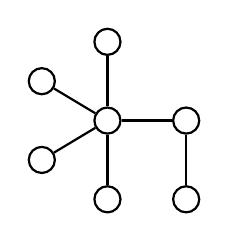
\begin{tikzpicture}[scale=1,
  thick,main node/.style={circle,draw,font=\sffamily\bfseries,minimum size=3mm}]

  \node[main node] (0) at (1/6,1/2) {};
   \node[main node] (1) at (1/6,3/2) {};
  \node[main node] (2) at (1,0){};
  \node[main node] (3) at (1,1){};
  \node[main node] (4) at (1,2) {};
  \node[main node] (5) at (2,0) {};
  \node[main node] (6) at (2,1) {};

  \path[every node/.style={font=\sffamily\small}]
     (0) edge node[above]{}(3)
   (1) edge node[above]{}(3)
   (2) edge node[above]{}(3)
   (3) edge node[above]{}(6)
   (4) edge node[above]{}(3)
   (5) edge node[above]{}(6);
\end{tikzpicture}
\end{wrapfigure}

\begin{thm}{Proposition}
Let $T$ be the bipolar tree as on the diagram.
If a Riemannian manifold satisfies the $T$-tree comparison for the tree on the diagram then it is CTIL.
\end{thm}

\parit{Proof.}
Assume contrary; that is, there is $p\in M$ and $u,v\in \TIL_p$ such that $w=\tfrac12\cdot(u+v)\notin \TIL_p$.

}

Let $\tau$ be the maximal value such that the geodesic $\gamma(t)=\exp_p(w\cdot t)$ is a length-minimizing on $[0,\tau]$.
Note that $\tau<1$ and $w'=\tau\cdot w\in\partial \TIL_p$; that is there is $w''\in\TIL_p$ such that $\exp_pw'=\exp_pw''$.



According to \cite{karcher}, for generic point on $z\in\partial \TIL_p$ there are at least two minimizing geodesics connecting $p$ to $q=\exp_p z$.
By general position argument we can assume that this is the case for $z=w'$.

\begin{wrapfigure}{r}{26 mm}
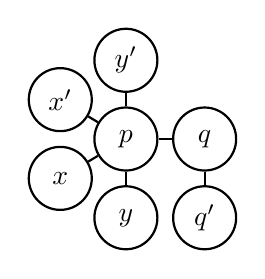
\begin{tikzpicture}[scale=1,
  thick,main node/.style={circle,draw,font=\sffamily\bfseries,minimum size=8mm}]

  \node[main node] (0) at (1/6,1/2) {$x$};
   \node[main node] (1) at (1/6,3/2) {$x'$};
  \node[main node] (2) at (1,0){$y$};
  \node[main node] (3) at (1,1){$p$};
  \node[main node] (4) at (1,2) {$y'$};
  \node[main node] (5) at (2,0) {$q'$};
  \node[main node] (6) at (2,1) {$q$};

  \path[every node/.style={font=\sffamily\small}]
     (0) edge node[above]{}(3)
   (1) edge node[above]{}(3)
   (2) edge node[above]{}(3)
   (3) edge node[above]{}(6)
   (4) edge node[above]{}(3)
   (5) edge node[above]{}(6);
\end{tikzpicture}
\end{wrapfigure}

It remains to produce an array of 7 points which fail the $T$-tree comparison.

Fix $\eps>0$, consider the points
\begin{align*}
q&=\exp_pw'=\exp_pw'',
&
q'&=\exp_p(\eps\cdot w''),
\\
x&=\exp_p u,
&
x'&=\exp_p (-\eps\cdot u),
\\
y&=\exp_p v,
&
y'&=\exp_p (-\eps\cdot v).
\end{align*}
Let us show that if $\eps$ is small, then the array $p,x,x',y,y',q,q'$ does not satisfy the $T$-tree comparison to the labeling as on the diagram.

Assume contrary; let $\~p,\~x,\~x',\~y,\~y',\~q,\~q'\in\HH$ be a point array as in the definition of $T$-tree comparison.
Note that ???
\qeds




